\documentclass{article} % For LaTeX2e
\usepackage{nips13submit_e,times}
%\documentstyle[nips12submit_09,times,art10]{article} % For LaTeX 2.09
%\newtheorem{observation}{Observation}
%\newtheorem{claim}{Claim}
%\newtheorem{conjecture}{Conjecture}
%\newtheorem{problem}{Problem}
%\newtheorem{algo}{Algorithm}
%\newtheorem{definition}{Definition}
%\newtheorem{lemma}{Lemma}
%\newtheorem{theorem}{Theorem}
%\newtheorem{proof}{Proof}
%\newtheorem{defi}{Definition}

\newcommand\independent{\protect\mathpalette{\protect\independenT}{\perp}}
\def\independenT#1#2{\mathrel{\setbox0\hbox{$#1#2$}%
\copy0\kern-\wd0\mkern4mu\box0}} 

\newcommand{\atiter}[2]{{#1}^{(#2)}}
\newcommand{\itert}[1]{{#1}^{(t)}}
\newcommand{\itertO}[1]{{#1}^{(t+1)}}
\newcommand{\iiter}[1]{{#1}^{(i)}}
% \newcommand{\raiseTheta}[1]{\theta^{#1}}
\newcommand{\raisePsi}[1]{\psi^{#1}}
\newcommand{\order}[1]{\mathcal{O}(#1)}

\newcommand{\hide}[1]{}
\newcommand{\comment}[1]{\textcolor{red}{{\small #1 }}}
\newcommand{\semihide}[1]{{\tiny #1}}
\newcommand{\reminder}[1]{{\textsf{\textcolor{red}{[#1]}}}}
\newcommand{\makeclean}{
    \renewcommand{\reminder}[1]{}
}

%\newcommand{\QED}{ \hfill {\bf QED}}
\newcommand{\tight}{ \setlength{\itemsep}{-1.0\itemsep} }
    % makes lists tighter

\usepackage[mathscr]{eucal} %% For \mathscr
\usepackage{amsbsy} %% For \boldsymbol
\newcommand{\tensor}[1]{\boldsymbol{\mathscr{#1}}}   %% Tensor macro from Tammy
% \newcommand{\tensor}[1]{{\boldmath\mathcal{#1}}}
\newcommand{\B}[1]{\mathbf{#1}}   %% Tensor macro from Tammy
%\newcommand{\tensor}[1]{\underline{\mathbf{#1}}}  
%\newcommand{\tensor}[1]{\mathbf{\EuScript{#1}}}  
%\newcommand{\tensor}[1]{\mathbf{\mathcal{#1}}}  
\newcommand{\loss}{\mathcal{L}}  

\newcommand{\krp}[2]{ \left( \mathbf{#1}\odot\mathbf{#2} \right)}

\def\blambda{\mbox{\boldmath ${\lambda}$}}

\newcommand{\method}{\textsc{METHOD}\xspace}
\newcommand{\methodplain}{METHOD\xspace}
\newcommand{\graphlab}{GraphLab\xspace}
\newcommand{\psgd}{PSGD\xspace}
\newcommand{\dsgd}{DSGD+\xspace}
\newcommand{\lda}{LDA\xspace}
\newcommand{\dl}{DL\xspace}
\newcommand{\mmsb}{MMSB\xspace}
\newcommand{\twitter}{TGraph\xspace}
\newcommand{\nytimes}{NyTimes\xspace}
\newcommand{\snytimes}[1]{NyTimes{#1}\xspace}
\newcommand{\scaleblenytimes}{Scalable NyTimes\xspace}
\newcommand{\pubmed}{PubMed\xspace}
\newcommand{\imagenet}{ImageNet\xspace}

\newcommand{\sgd}{SGD\xspace}

%\newcommand{\explosion}{\textsc{Idex}\xspace}
\newcommand{\explosion}{intermediate data explosion\xspace}
\newcommand{\Explosion}{Intermediate Data Explosion\xspace}
\newcommand{\gtscaleup}{100\xspace}

\newcommand{\samplecube}{\textsc{ParCube}\xspace}
\newcommand{\parafac}{\textsc{Parafac}\xspace}
\newcommand{\sparafac}{\textsc{Parafac SLF}\xspace}
\newcommand{\merge}{\textsc{Merge}\xspace}
\newcommand{\sample}{\textsc{BiasedSample}\xspace}
\newcommand{\enron}{\textsc{Enron}\xspace}
\newcommand{\facebook}{\textsc{Facebook}\xspace}
\newcommand{\lbnl}{\textsc{Lbnl}\xspace}
\newcommand{\nell}{\textsc{Nell}\xspace}
\newcommand{\argmin}{\text{argmin}\xspace}
\newcommand{\brain}{\textsc{BrainQ}\xspace}


\newcommand{\hadi}{{\cal HADI}\xspace}
\newcommand{\mapreduce}{\textsc{MapReduce}\xspace}
\newcommand{\map}{\textsc{Map}\xspace}
\newcommand{\reduce}{\textsc{Reduce}\xspace}
\newcommand{\combine}{\textsc{Combine}\xspace}
\newcommand{\hadoop}{\textsc{Hadoop}\xspace}
\newcommand{\anf}{\emph{Centralized Method}}
% \newcommand{\MFB}{{MF-bitstring}}
\newcommand{\MFB}{{FM-bitstring}}
\newcommand{\mfb}{{b}}
\newcommand{\MFV}{{FM-vector}}
\newcommand{\mfv}{{\bf v}}
% \newcommand{\mfbhi}{{MF-vector}}
\newcommand{\mfbhi}{{ b(h,i) }}
\newcommand{\Nhi}{N(h,i)}   % number of neighbors of $i$, within h hops or less
\newcommand{\NNhi}{ {\cal N}(h,i)} % SET of neighbors ....
\newcommand{\NNhhi}{ {\cal N}(h+1,i)} % SET of neighbors ....
\newcommand{\NNhj}{ {\cal N}(h,j)} % SET of neighbors ....
\newcommand{\hatmfbhi}{ $\hat{b}(h,i)$} %partial bitmask

\newcommand{\PassA}{{\tt Stage1}\xspace}
\newcommand{\PassAMap}{{\tt Stage1-Map}\xspace}
\newcommand{\PassARed}{{\tt Stage1-Reduce}\xspace}
\newcommand{\PassB}{{\tt Stage2}\xspace}
\newcommand{\PassBMap}{{\tt Stage2-Map}\xspace}
\newcommand{\PassBRed}{{\tt Stage2-Reduce}\xspace}
\newcommand{\PassC}{{\tt Stage3}\xspace}
\newcommand{\PassCMap}{{\tt Stage3-Map}\xspace}
\newcommand{\PassCRed}{{\tt Stage3-Reduce}\xspace}

\newcommand{\diameter}{{\tt diameter}}
\newcommand{\npairs}{{\tt npairs}}
\newcommand{\gcc}{{\tt gcc}}
\newcommand{\entropy}{{\tt entropy}}
% \newcommand{\nedges}{{\tt nedges}}
\newcommand{\sv}{{\mbox{$\lambda_1$}}}
\newcommand{\avgd}{{\tt avgd}}

% math symbol definitions
\newcommand{\mat}[1]{{\bf{#1}}}
\newcommand{\nnodes}{N}     % number of nodes
\newcommand{\nedges}{E}     % number of edges
\newcommand{\deff}{{d_{eff}}}   % effective diameter
\newcommand{\Er}{{E_{r}}}   % number of retained edges
\newcommand{\Nr}{{N_{r}}}   % number of retained nodes
\newcommand{\Nc}{{N_c}}   % number of nodes at critical point
\newcommand{\Ec}{{E_c}}   % number of nodes at critical point
\newcommand{\Ngcc}{{N_{gcc}}} % number of nodes in gcc, at critical poing
\newcommand{\NPairc}{{N_{NPAIRS}}} % number of reachable pairs, at critical poing
\newcommand{\dc}{{d_{c}}} % diameter at critical point
\newcommand{\Lambdac}{{\lambda_{c}}} % First eigenvalue at critical point
% \newcommand{\RED}{ {\em RED } } % random edge deletion
% \newcommand{\FED}{ {\em FED } } % friendly edge deletion
% \newcommand{\HED}{ {\em HED } } % hostile edge deletion
\newcommand{\join}{\texttt{combine2}}
\newcommand{\aggrnp}{\texttt{combineAll}}
\newcommand{\aggr}{\texttt{combineAll$_i$}}
\newcommand{\aggrsid}{\texttt{combineAll$_{E.sid}$}}
\newcommand{\assign}{\texttt{assign}}



\newcommand{\ben}{\begin{enumerate*}}
\newcommand{\een}{\end{enumerate*}}
\newcommand{\bit}{\begin{itemize*}}
\newcommand{\eit}{\end{itemize*}}

% shorthands
\newcommand{\citationsds}{{CITATIONS}}
\newcommand{\epinionsds}{{EPINIONS}}
\newcommand{\patentsds}{{PATENTS}}
\newcommand{\net}[1]{{\textsc{#1}}}

\newcommand{\QED}{\hfill $\Box$ \hfill}





% graph segment
% Notation macros
\newcommand{\G}{\ensuremath{{\mathcal G}}}  % graph stream
\newcommand{\ES}[1]{\ensuremath{m^{(\!#1\!)}}}
%\newcommand{\ES}[1]{\ensuremath{|E|^{(\!#1\!)}}}
\newcommand{\coll}{\ensuremath{\ell}}  % number of source/row groups
\newcommand{\rowk}{\ensuremath{k}}  % number of dest/col groups
\newcommand{\rgrp}[1]{\ensuremath{I^{(\!#1\!)}}}  % node set for src/row group
\newcommand{\cgrp}[1]{\ensuremath{J^{(\!#1\!)}}} % node set for dst/col group
\newcommand{\rgsz}[1]{\ensuremath{l^{(\!#1\!)}}}  % size of node set for src/row group
\newcommand{\cgsz}[1]{\ensuremath{n^{(\!#1\!)}}  }% size of node set for dst/col group
\newcommand{\subG}[1]{\ensuremath{{\mathcal G}^{(\!#1\!)}}}  % submatrices
\newcommand{\den}[1]{\ensuremath{\rho^{(\!#1\!)}}}   % density/probability
\newcommand{\KL}[2]{\ensuremath{{\mathcal D}(#1\|#2)}}   % KL-divergence
\newcommand{\ceil}[1]{\ensuremath{\lceil\!#1\!\rceil}}   % density/probability

\newcommand{\myrot}[1]{\rotatebox[origin=ll]{75}{{#1}}} 


\usepackage{amsmath}%,amsthm}
\usepackage{amsfonts}
\usepackage{amssymb}
\usepackage{subfigure, fink, grffile, placeins}
\usepackage[pdftex]{graphicx} 
\usepackage{epstopdf}
\usepackage{hyperref}
% \usepackage[colorlinks,pagebackref]{hyperref}
% \usepackage[pagebackref]{hyperref}
%\usepackage[usenames,dvipsnames]{xcolor}
%\usepackage{algorithmicx,algpseudocode,algorithm}
\usepackage[lined,boxed]{algorithm2e}
\usepackage{url}
% \usepackage[boxed,noend]{algorithm2e}
%\usepackage{mdwlist}    % from christos / mary: makes lists tighter
%\usepackage{epsfig}
%\usepackage{times}
%\usepackage{setspace}
%\usepackage[pdftex]{graphicx}
%\usepackage[pdftex]{geometry}

%\usepackage{algorithm}
%%\usepackage{algorithmic}
%\usepackage{algpseudocode}
%\usepackage{program}


\newtheorem{observation}{Observation}
\newtheorem{conjecture}{Conjecture}
\newtheorem{problem}{Problem}
\newtheorem{algo}{Algorithm}
\newtheorem{definition}{Definition}
\newtheorem{lemma}{Lemma}
\newtheorem{theorem}{Theorem}
\newtheorem{assumption}{Assumption}
%\newtheorem{question}{Question}
\newtheorem{example}{Example}
\newcommand{\pushright}[1]{\ifmeasuring@#1\else\omit\hfill$\displaystyle#1$\fi\ignorespaces}
\newcommand{\pushleft}[1]{\ifmeasuring@#1\else\omit$\displaystyle#1$\hfill\fi\ignorespaces}
%\newtheorem{answer}{Answer}
%\newtheorem{proof}{Proof}

\newcommand{\abhi}[1]{\textcolor{orange}{abhi-comment: #1}}
\newcommand{\alex}[1]{\textcolor{red}{\\ alex-comment: #1}}
\newcommand{\qirong}[1][1]{\textcolor{fuschia}{\\ qirong-comment: #1}}
\newcommand{\eric}[1][1]{\textcolor{blue}{\\ eric-comment: #1}}

\title{Slow-Worker-Agnostic Distributed Learning for Big Models on Big Data}
%\title{Slow-learner ain't My Problem: Stochastic Learning for Big Models on Big Data}
%\title{Slow-learner ain't My Problem: Exploiting Structure in high-D, high-V Latent Space Stochastic Learning}
% \title{Community Discovery through Optimization}


\author{
% Abhimanu Kumar~~~~~~Alex Beutel~~~~~~Qirong Ho~~~~~~Eric P. Xing 
% \\ School of Computer Science, Carnegie Mellon University 
% \\ Pittsburgh PA 15213,USA,\\
% \{\href{mailto:abhimank@cs.cmu.edu}{abhimank},\href{mailto:abeutel@cs.cmu.edu}{abeutel},
% \href{mailto:qho@cs.cmu.edu}{qho},
% \href{mailto:epxing@cs.cmu.edu}{epxing}\}@cs.cmu.edu
}


% \authorrunning{Kumar et al.}
% The \author macro works with any number of authors. There are two commands
% used to separate the names and addresses of multiple authors: \And and \AND.
%
% Using \And between authors leaves it to \LaTeX{} to determine where to break
% the lines. Using \AND forces a linebreak at that point. So, if \LaTeX{}
% puts 3 of 4 authors names on the first line, and the last on the second
% line, try using \AND instead of \And before the third author name.

\newcommand{\fix}{\marginpar{FIX}}
\newcommand{\new}{\marginpar{NEW}}

%\nipsfinalcopy % Uncomment for camera-ready version

% Use this to modify float spacing
%\setlength\textfloatsep{20pt plus 2pt minus 4pt}

\begin{document}


\maketitle

\begin{abstract}
We present a scheme for fast, distributed learning on
big (i.e. high-dimensional) models applied to big datasets.
Unlike algorithms that focus on distributed learning in either the big data or big model setting
(but not both), our scheme partitions both the data and model variables
simultaneously. This not only leads to faster learning on distributed clusters,
but also enabes machine learning applications where both data
and model are too large to fit within the memory of a single machine. Furthermore, our scheme
allows worker machines to perform additional updates while waiting for slow workers to finish,
which provides users with a tunable synchronization strategy that can
be set based on learning needs and cluster conditions.
We prove the correctness of such strategies, as well as provide
bounds on the variance of the model variables under our scheme.
Finally, we present empirical results for latent space models such
as dictionary learning and topic models, which demonstrate that our method
scales well with large data and model sizes, while beating
learning strategies that fail to take model partitioning into account.

%	We present here a scheme for exploiting distributable structure present in
%	latent space model for high-dimensional (high-D) and high-volume (high-V)
%	learning. Models like latent dirichlet allocation, mixed membership
%	stochastic blockmodels, dictionary learning have structures that can be
%	exploted for big learning.
%	We present a distributed learning strategy for such models. The scheme is
%	distributed in data as well as parameter space and avoids waiting for slow
%	learners to obtain full distributive leverage.
%	The learning scheme, flexible to slow worker-processors, has
%	provably correct strategy for convergence even with fewer synchronizations.
%	It provides a tunable synchronization startegy that can be set based on the
%	learning needs and system quality with the end user. We provide theoretical
%	bounds on the parameter variance among workers with different synchronization 
%	strategies. Empirical
%	results presented for latent space models such as latent dirichlet allocation 
%	and dictionary learning show that it scales very well with large data
%	as well as parameter space. The comparative evaluation with other parallel
%	and distributed learning startegies shows better preformance of the model.	
\end{abstract}

\vspace{-0.3cm}
\section{Introduction}
\vspace{-0.3cm}

Machine Learning applications continue to grow rapidly, in terms of both input
data size (big data) as well as model complexity (big models). The big data challenge
is already well-known --- with some estimates putting the amount of data generated on the internet
at 5 exabytes every two days~\footnote{\url{http://techcrunch.com/2010/08/04/schmidt-data/}} ---
and much effort has been devoted towards learning models on big datasets, particularly through
stochastic optimization techniques that randomly partition the data over different machines. Such techniques
have been the subject of much theoretical
scrutiny~\cite{langford2009slow,zinkevich2010parallelized,agarwal2012distributed,hoffman2012stochastic}.
On the other hand, the big model issue is about learning models with an extremely large number of variables
and/or parameters --- such as the Google Brain deep network with over 1B parameters~\cite{dean2012large} ---
and recent papers on this subject have focused on intelligent partitioning of the model variables in
order to minimize network synchronization costs~\cite{low2012distributed,dean2012large}, albeit not always
with theoretical backing.

Although big data and big models are both crucial research foci, there are few
distributed machine learning papers that explicitly consider both aspects in conjunction, with a notable example
being the partitioned matrix factorization algorithm of Gemulla {\it et al.}~\cite{Gemulla:2011:LMF:2020408.2020426}. In the big data,
big model setting, the model variables may not all fit into a single machine's memory, which in turn imposes
additional constraints on how the data is partitioned. Moroever, careless partitioning of model variables
across distributed machines imposes significant network synchronization costs~\cite{low2012distributed}, which
are required whenever dependent variables or datapoints are placed on separate machines.
If we are to effectively partition both data and model, it follows that we must carefully
examine and exploit the interdependencies between data and model variables.

In this paper, we address learning big latent space models on big data over a distributed cluster.
Specifically, we develop and theoretically analyze a stochastic optimization algorithm for learning latent space models that can be
expressed in matrix form, such as dictionary learning or topic modeling. Our algorithm exploits the
matrix structure to partition the data and model variables over a distributed cluster, in a manner
that automatically balances inter-machine network synchronization costs with performing useful computational work,
even when the worker machines are not equally capable (e.g. because of different hardware or other
concurrently running programs), or the data cannot evenly partitioned (e.g. due to the structure of the model).

As a result, our algorithm solves the ``last reducer" issue in Hadoop clusters, in which some worker machines
can be much slower than others (because of cluster heterogeneity, or because other jobs are running on the same
machine), causing faster workers to waste computational cycles waiting for them.
Instead, we ensure that faster workers will continue to perform
useful work until the last reducer finishes, and our theoretical and experimental analysis confirms that this
strategy leads to faster algorithm convergence. Furthermore, our theory shows that careful control of inter-worker
synchronization can lead to even faster convergence, which opens the door to intelligent exploitation
of distributed computation systems with better fine-grained synchronization than Hadoop, such
as parameter servers~\cite{cipar2013solving,ahmed2012scalable,power2010piccolo}.


%In todays information age there is trillions of bytes of data being generated
%every moment. By one estimate we generate 5 exabytes of data on the internet every two
%days~\footnote{\url{http://techcrunch.com/2010/08/04/schmidt-data/}} 
%and most of
%it is user generated content. Given this massive amount of data generated
%every moment large scale machine learning is not just of academic
%interest anymore but of practical significance too. Large scale learning or big
%learning has been an active area of research in recent times. But most of this
%research has been focused around big data and the aspect of distibuting the
%learnig model has take back seat. While dealing with big data is definitely a must in this massive
%content generation age the learning task might turn out to be non-trivial when
%big data meets complex models. Learning models with high dimension or number of
%parameters becomes non-trivial even with slight increase in data. 
%Hence there is a need for learning scheme which can perform distributed data as
%well as parameter learning. This problem is highly prevalent in latent space 
%model such as latent dirichlet allocation (LDA~\cite{Blei:2003:LDA}), mixed
%membership stochastic blockmodels (MMSB~\cite{Airoldi:2008:MMS}) as they inflate
%their parameter space by introducing large number of latent variables.
%Henceforth these models would be our object of focus in this paper. We develop a
%stochastic learning scheme for latent space model, specifically for LDA and
%MMSB, which is distributed in data as well as parameter space. We modify the
%originial objective to suit our optimization scheme.\comment{need to write this
%in a better way}. The structure obtained can be further exploited to minimize
%the hazardous effects of slow-processors in the distributed system.  
%
%\comment{expand some more giving an over view of our learning scheme}

\vspace{-0.3cm}
\section{Related Work}
\vspace{-0.3cm}

%\comment{Qirong: We may want to move related work to the back. The related work section
%usually makes more sense to the reader after he/she understands our approach.}
%
%\comment{Qirong: Note that the related work section is for discussing the high-level picture,
%and not deep theoretical connections. Those should be relegated to the theory section.
%We want to keep paper accessible to a non-theory audience.}
%
%\comment{Qirong: Given that our latent space modeling is only a secondary contribution
%(the primary contribution being big data+model learning), it should only be discussed
%in the experiments section.}

Most existing literature is focused on learning under either big data or big model conditions, but
rarely both together. Of the papers that focus on big data, most of them exploit data point
indepedence to construct stochastic distributed optimization schemes with little need
for inter-machine synchronization. For example, the PSGD algorithm~\cite{zinkevich2010parallelized}
is completely data parallel and requires absolutely no inter-machine communication,
therefore making it trivial to implement. This fact is only of academic interest however --- in practice,
one can almost always obtain faster convergence with some inter-machine communication, as our experiments show.
Another important class of methods are the fixed-delay algorithms~\cite{agarwal2012distributed,langford2009slow} in which machines communicate
with a central server (or each other) in a fixed ordering. This fixed ordering is a serious practical limitation,
because all machines will be held up by slowdowns or failures in just one machine.
In contrast, our algorithm ensures that all machines continue to do useful work even under such conditions.
Most importantly, unlike these big data algorithms, our algorithm can partition model variables
(and not just datapoints) across machines, which is absolutely critical for massive models that cannot fit onto a single machine.

For learning on big models, the general strategy is to exploit the fact that each model variable usually
depends on only a small number of other variables, and then partition model variables
in a way that limits the number of dependencies that cross machines. The GraphLab system~\cite{low2012distributed}
is a good example of this concept, but it requires machine learning algorithms to be rewritten into
``vertex programs", which can be awkward or even difficult for some algorithms. Furthermore,
there has been little theoretical analysis on machine learning algorithms running under GraphLab.
The Google Brain project~\cite{dean2012large} provides another example of the need for model partitioning,
this time for a custom-built deep network meant for image and video feature extraction. However, the
paper does not provide general partitioning strategies for arbitrary models. Finally, we note that
the Hogwild paper~\cite{niu2011hogwild} provides a theoretical analysis of certain issues related to model partitioning ---
specifically, the effect of errors produced when two worker threads update the same variable simultaneously.
Aside from that, the paper does not provide or analyze any model partitioning strategies whatsoever, and the
experiments only cover the shared-memory, single-machine setting.

Finally, there are papers that tackle big data and big model issues together, such as the partitioned matrix factorization
algorithm of Gemulla {\it et al.}~\cite{Gemulla:2011:LMF:2020408.2020426}, to which our work is most closely related. Unlike Gemulla {\it et al.},
our algorithm allows worker machines to perform useful variable updates continuously, without blocking or waiting
for any other machine to complete its assigned task. This property is exceptionally beneficial
on very large clusters, where machines often fail or slow down for any number of reasons. Thus, our algorithm
is not bottlenecked by the slowest machine, unlike~\cite{Gemulla:2011:LMF:2020408.2020426}. Furthermore, we provide substantially
richer theoretical analysis, including variance bounds and analysis of the effect of non-blocking workers.

%Not necessary, in the ML community, citing recent papers is more important
%\comment{Theory work: Write couple of lines about Stochastic Approximation book and Noboru Murata's analysis}

%\comment{Qirong: Are my claims about our theory correct? Just want to confirm}

%\comment{PSGD (only data parallel); Aggarawal and Duci's Distributed Delayed
%(Again Data partition only; and it's hard to code); Any Other?}
%\comment{How do we discuss the original Haas's paper though we do considerable
%more in terms of theory and multi-iteration}
%\comment{Theory work: Stochastic Approximation book; Zinkevich, Noboru Murata}

\vspace{-0.3cm}
\section{Slow-Worker Agnostic Learning for Big Models on Big Data}
\vspace{-0.3cm}

Our approach to learning big models on big data relies on
exploiting independent cliques of structure.
For example, a probabilistic graphical model might contain a massive
number of latent variables and parameters,
so as to capture the modeler's generative assumptions about large datasets.
%Though this enables these models with a unique ability to provide an interpretation and a generative story,
%it also makes the model harder to learn since the parameter as well as variable space increases
%massively. These models when run on large data have their learning problem become twice difficult. 
%While it may appear that latent space models' biggest boon
%of incorporating hidden variables is their biggest bane for large scale
%learning, it turns out that is not the case.
In order to tackle problems of such scale, we need to exploit independence structures
present in the data and model, so as to partition both over a distributed cluster.

Before we detailing our partitioning strategy, we shall present some example ML problems.
Consider {\bf Topic Modeling}~\cite{blei2009topic}: given a \emph{ document by vocabulary} data matrix $Y$ (with the
rows normalized to sum to 1),
we want to decompose it into two matrices: \emph{ documents by topics} $\pi$ (which are model variables) and
\emph{ topics by vocabulary} $\beta$ (which are parameters). We formulate this task
as an optimization problem with simplex and non-negativity constraints:
\vspace{-0.1cm}
\begin{align}
\argmin_{\pi,\beta}L(Y,\pi,\beta) =||Y-\pi\beta||_p^p = \sum_{i,j}(Y_{i,j}-\sum_k
\pi_{i,k}\beta_{k,j})_p^p \label{eqn:LDA}\\
\text{s.t.} \; \forall  i,j,k \quad
\sum_k\pi_{i,k}=1, \quad
\sum_j\beta_{k,j}=1, \quad
\pi_{i,k}\geq 0, \quad
\beta_{k,j}\geq 0,
\nonumber
\end{align}
where $\Vert \cdot \Vert^P_P$ is an $\ell_p$ norm, typically $\ell_2$. We note
that other matrix-decomposition-based algorithms for topic modeling also exist, such
as the spectral decomposition method of Anima {\it et al.}~\cite{anandkumar2012two}.
%For MMSB a similar objective can be formulated. Given a \emph{ user by user}
%adjacency matrix $Y$ it aims to find
%two matrices $\pi$ and $B$, which are \emph{user by topic} and \emph{topic by
%topic} matrix respectively, such that $\pi^TB\pi$ reconstructs the original
%matrix interaction matrix $Y$. Equation~\ref{eqn:MMSB} presents this in an
%optimization framework with the usual non-negativity and simplex constraints. 
%\begin{eqnarray}
%\argmin_{\pi,B}L=||Y-\pi^TB\pi||_p^p = \sum_{i,j}(Y_{i,j}-\sum_{g,h}
%\pi_{i,g}B_{g,h}\pi_{j,h})_p^p \label{eqn:MMSB}\\
%s.t.\sum_k\pi_{i,k}=1,\pi_{i,k}\geq 0, B_{i,k}\geq 0~~\forall~ i,j \nonumber
%\end{eqnarray}
Another problem is {\bf Dictionary Learning}~\cite{Kreutz-Delgado:2003:DLA},
in which the goal is to decompose a signal matrix $Y$ into a dictionary $D$
and a sparse reconstruction $\alpha$:
\vspace{-0.1cm}
\begin{align}
\argmin_{\alpha,D} L(Y,D,\alpha) =\frac{1}{2}||Y-D\alpha||_2^2 + \lambda||\alpha||_1
\qquad\qquad
\text{s.t.} \; \forall j, \quad D_j^TD_j \leq 1
\label{eqn:dictionary}
\end{align}
%  \comment{Do we present the symmetric matrix
% factorization objective too; since it's is nice scheduling scheme 
% as well as $\ell_p$ and $\ell_2$ combined loss}
Compared to unconstrained Matrix Factorization (MF) and Non-negative MF (NMF) tasks, latent space
models usually feature more constraints: simplex constraints in the case of topic modeling, and
bounded inner product in the case of dictionary learning. In order to handle these constraints,
our distributed learning algorithm supports projection steps to ensure the final solution always
satisfies the constraints.
We note that while many recent distributed algorithms have theoretical guarantees
under projection~\cite{langford2009slow,agarwal2012distributed,Gemulla:2011:LMF:2020408.2020426},
some algorithms such as PSGD~\cite{zinkevich2010parallelized} do not explicitly handle projections,
and are thus unsuitable for the latent space models defined above.

%\comment{Qirong: Abhi, do you know of any other algorithms without projection guarantees?
%Just having PSGD makes it look like projections are nothing special}

\vspace{-0.2cm}
\subsection{Partitioning Strategy and Distributed Algorithm}
\vspace{-0.2cm}

\begin{figure}[t]
\vspace{-0.5cm}
\centering
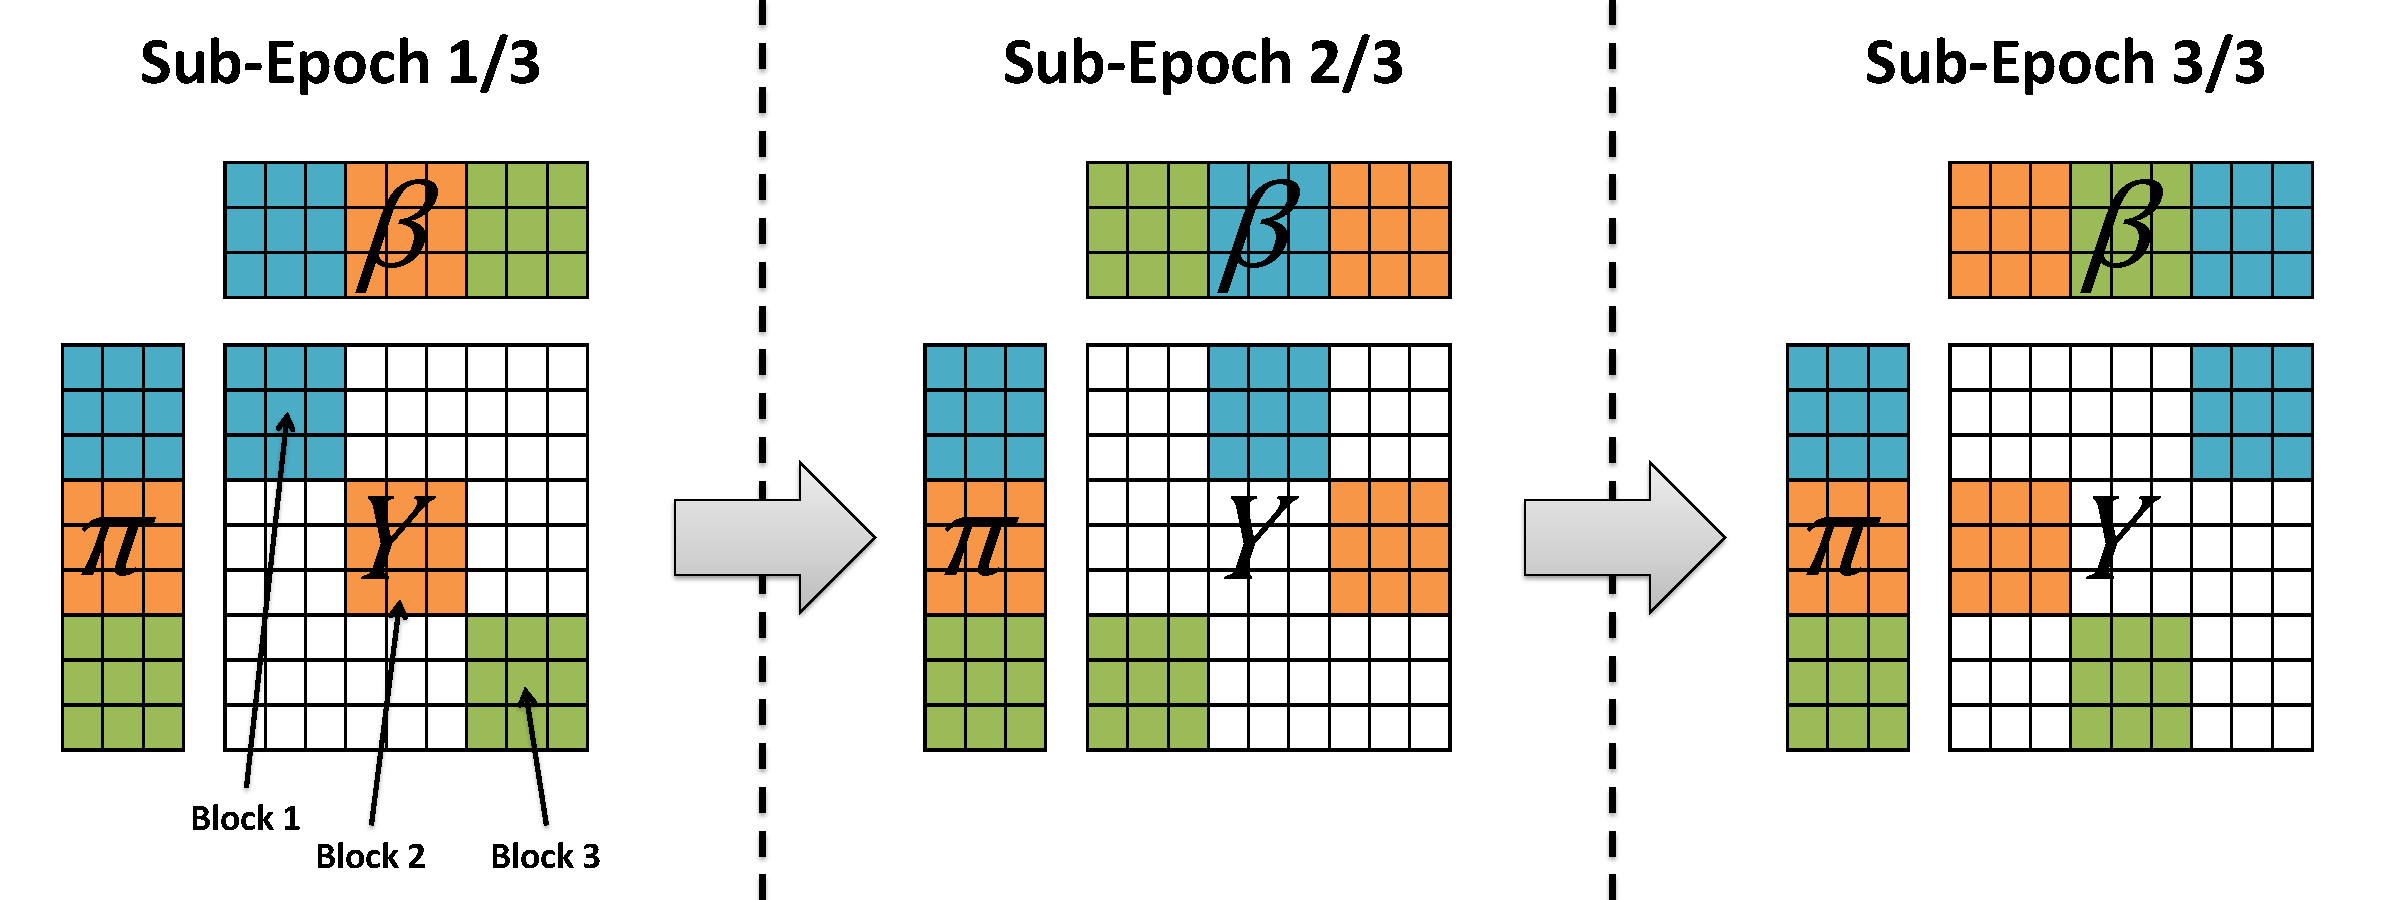
\includegraphics[width=\textwidth]{fig/partition.pdf}
\vspace{-0.6cm}
\caption{\small Partitioning strategy for data $Y$, model variables $\pi$, and parameters $\beta$.
We show one epoch broken into multiple sub-epochs (3 in this case).
Each sub-epoch is further divided into (colored) blocks, such that the data $Y_{i,j}$ (with its
associated variables $\pi_{i,\cdot}$ and parameters $\beta_{\cdot,j}$) from one block do not
share rows/columns with data $Y_{a,b}$ from another block. Taken together, all blocks from
all sub-epochs cover every element of $Y,\pi,\beta$.
}
\label{fig:para-div}
\vspace{-0.5cm}
\end{figure}

\paragraph{High-level overview}
In order to solve these problems effectively on a distributed cluster,
we need to exploit the interdependence of parameters and variables.
For example, consider the topic modeling objective $L(Y,\pi,\beta)$:
we can divide the data matrix $Y$ into a sequence of sub-epochs, where
each epoch consists of blocks that do not overlap on parameters $\beta$ and variables $\pi$,
and where the union over all epochs covers the entire matrix (Figure~\ref{fig:para-div}).
This blocking strategy is attributed to Gemulla {\it et al.}~\cite{Gemulla:2011:LMF:2020408.2020426}, and it
permits multiple machines to perform stochastic gradient descent (SGD) on different blocks in parallel,
on a Hadoop cluster. However, it requires all workers to process a roughly equal number of datapoints
per block, which leads to problems with slow workers. Our algorithm and theoretical analysis removes this limitation,
allowing faster workers to process extra datapoints in their assigned block, which maximizes
the cluster's computational efficiency.

At a high level, our algorithm proceeds one epoch at a time,
performing SGD on all blocks within an epoch in parallel.
In order to satisfy the problem constraints, we must interleave projection steps with
the SGD algorithm. In this respect, the parameters $\beta$ and variables $\pi$ 
must be handled differently: while the simplex projection for variables $\pi$ can
be performed by each worker independently of others,
the simplex projection for the parameters $\beta$ requires workers to repeatedly synchronize with each other.
This cannot be done through the MapReduce programming model, so our Hadoop implementation allows workers
to write to the Hadoop Distributed File System (HDFS) in order to communicate projection information with each other.
We find that this scheme works well in practice, while dedicated, memory-based synchronization systems such as
parameter servers~\cite{cipar2013solving,ahmed2012scalable,power2010piccolo} have the potential to perform even better.

\vspace{-0.2cm}
\paragraph{Partitioning strategy}
More formally, let $\bold{\Psi}$ collectively refer to the variables and parameters
$\mathbf{\pi, \beta}$, and let $\psi$ refer to individual elements of $\bold{\Psi}$.
These definitions will make the subsequent analysis easier to understand.
Thus, we rewrite the LDA objective $L$ as: 
%(\comment{note:projections are involved here})
\vspace{-0.1cm}
\begin{align}
\psi^{(t+1)}&= \psi^{(t)} - \eta_t \nabla
\loss_{Y_{i,j}}(\psi^{(t)}),
\label{equ:sgd-update-lda}
\end{align}
and we apply parameter/variable projections each time we execute Eq.~(\ref{equ:sgd-update-lda}).
Assuming that we use the $\ell_2$ norm, the differential of $\psi$ with respect
to $\pi$ at a single data point $Y_{i,j}$ is
\vspace{-0.1cm}
\begin{align}
	(\nabla L_{Y_{i,j}}(\psi))_\sigma &= 
	\left\{
	\begin{array}{ll}
		-2(Y_{i,j}-\sum_k \pi_{i,k}\beta_{k,j}
		)\beta_{\ell,j}  & \mbox{if } \sigma = \pi_{i,\ell} \\
		0 & \mbox{if } \sigma = \pi_{i',\ell},\ i\neq i'\\
	\end{array}
	\label{eqn:diff-lda}
\right.
\end{align}
where $\sigma$ is the element of $\pi$ being differentiated, and $(\nabla L_{Y_{i,j}}(\psi))_\sigma = \frac{\partial L_{Y_{i,j}}}{\partial \sigma}$.
The differentials with respect to $\sigma = \beta_{j,\ell}$, or even those for the dictionary learning problem, are similar.
From these equations, we observe that the SGD update for $\pi_{i,\ell}$ at a particular datapoint
$Y_{i,j}$ depends only on a small subset of the variables and parameters: specifically,
$\pi_{i,k}, \beta_{k,j}$ where $k\in {1,\ldots,K}$ and $K$ is the number of topics we chose.
Notice that the $\pi$ all come from the same row $i$ as $Y_{i,j}$, while the $\beta$ all come
from the same column $j$.
Furthermore, the SGD updates for $\pi_{i,\ell}$ are zero for any datapoint $Y_{a,b}$ where $a \ne i$.
A similar observation holds for the parameters: the SGD update for $\beta_{r,j}$ is zero for
any datapoint $Y_{a,b}$ where $b\ne j$.
%\comment{modify here for MMSB}

These observations lead to the following key insight: we can perform SGD on two datapoints $Y_{i,j}$ and $Y_{a,b}$ at the same
time, provided $i \ne a$ and $j \ne b$ --- in other words, as long as the datapoints do not
overlap on their rows or columns. An intuitive proof goes like this: SGD updates on $Y_{i,j}$ only touch the variable row $\pi_{i,\cdot}$
and the parameter column $\beta_{\cdot,j}$, and both of them do not overlap with $Y_{a,b}$'s variable row $\pi_{a,\cdot}$ and
parameter column $\beta_{\cdot,b}$. In other words, the SGD updates on $Y_{i,j}$ and $Y_{a,b}$
touch disjoint sets of variables $\pi$ and parameters $\beta$.
Furthermore, each $\pi_{i,\cdot}$ in row $i$ only ever depends on other $\pi$ in the same row $i$,
and similarly for $\beta_{\cdot,j}$ and other $\beta$ in column $j$. We therefore conclude that
all quantities associated with row $i$ and column $j$, namely $Y_{ij},\pi_{i\cdot},\beta_{\cdot j}$, are completely
independent of the quantities from row $a$ and column $b$, namely $Y_{ab},\pi_{a\cdot},\beta_{\cdot b}$.
Hence, datapoints with disjoint rows and columns can be simultaneously used for SGD updates~\cite{Gemulla:2011:LMF:2020408.2020426}.

From the perspective of data, model and parameter partitioning, we have essentially partitioned datapoints
$Y$, model variables $\pi$ and parameters $\beta$ into independent collections $(i,j)$ where
$i$ is a row index and $j$ is a column index. In other words, the collection $(i,j)$ contains $Y_{ij},\pi_{i\cdot},\beta_{\cdot j}$,
and can be ``processed" (meaning that we run SGD on $Y_{ij}$ to update $\pi_{i\cdot}$ and $\beta_{\cdot j}$)
in parallel with any other collection $(a,b)$ where $a\ne i$, $b \ne j$.

\vspace{-0.2cm}
\paragraph{Distributed algorithm}
Since collections $(i,j)$ with disjoint rows/columns can be processed
simultaneously, let us consider grouping
them into multiple blocks $S_b \subseteq Y$, such that the blocks have disjoint rows/columns (Figure~\ref{fig:para-div}).
While we cannot process collections $(i,j)$
within the same block in parallel (because they might share rows/columns), we can process collections from
{\it different} blocks in parallel, as they are guaranteed to be non-overlapping. Thus, if we managed to
construct $P$ non-overlapping blocks, we can spawn $P$ workers to perform SGD in parallel. Although it
is impossible to find a set of non-overlapping blocks that covers all of $Y$, we can find multiple disjoint sets of
non-overlapping blocks that, taken together, cover $Y$ completely (Figure~\ref{fig:para-div}). We call
these sets {\it sub-epochs}, which are processed sequentially (while the blocks within a sub-epoch
are processed in parallel). An {\it epoch} is a sequence of sub-epochs that fully covers $Y$.

%Given these update rules, we want to partition our data (and as a consequence, our model)
%into blocks $S_b \subseteq Y$ that can be run in parallel. Our partitioning strategy is shown in
%Figure \ref{fig:para-div}: we divide $Y$ into blocks such that no two
%blocks share common rows or columns.
%To be more precise, we say that a point
%$y \in S_b$ is the coordinates in the data, such as $y = (y_i,y_jy) \in
%Y$.  Two blocks $S_b$ and $S_{b'}$ are non-overlapping if
%for all $y \in S_b$ and
%$y' \in S_{b'}$, $y_i \neq y'_i$ and $y_j \neq y'_j$.
%Define a {\it sub-epoch} to be a set of pairwise row/column-disjoint blocks,
%and observe that in order to cover all regions of $Y$, we require multiple sub-epochs.
%Our algorithm runs the sub-epochs sequentially, and within each sub-epoch,
%we run SGD on the blocks in parallel. The order in which sub-epochs are
%run does not matter, as long as each sub-epoch is run once per epoch (defined
%as one pass over all blocks in $Y$).

Up to this point, our algorithm is similar to Gemulla~{\it et al.}. Where we differ
is that within a sub-epoch, we allow different worker-blocks to perform varying numbers of SGD updates per collection $(i,j)$
(whereas Gemulla~{\it et al.} require workers to perform equal amounts of SGD updates).
This makes our algorithm much more efficient whenever there are slow
worker machines (which tend to be the norm rather than the exception for large clusters),
since faster workers can keep running until synchronization, rather than
wasting computational cycles waiting for slower workers to catch up. Our full algorithm is shown in Algorithm \ref{algo:lda},
and in the next section, we shall prove that it converges, along with several other important properties.

Finally, we note that while this row/column-wise partitioning strategy for data/variables/parameters
happens to work for topic models and dictionary learning, it does not apply to all possible ML models:
for example, graphical models and deep networks can have arbitrary structure between parameters and variables,
while problems on time-series data will have sequential or autoregressive dependencies between datapoints.
In such cases, a row/column-wise partitioning will not work. Nevertheless, the {\it idea} and basic theoretical analysis of
grouping data, variables and parameters into independent collections still holds; only the partitioning
strategy needs to be changed. This opens up rich possibilities for future work on general-purpose partitioning algorithms
under our framework.

\IncMargin{1em}
\begin{algorithm}[t]
\small
\SetAlgoLined
Input : $Y,\beta, \pi$,~sub-epoch~size~$d$\\
$\pi\leftarrow \pi_0$, $\beta\leftarrow \beta_0$\\
Block $Y,\pi,\beta$ into corresponding $w$ blocks\\
\While{not converged}{
Pick step size $\eta_S$\\
% 	\For{$s=0,...,d^2-1$}{
%		\\\*sub-epoch\*\\\\
		Pick $w$ blocks($S_{1},...,S_{w}$) to form sub-epoch $S$\\
		\For{$b=0,\ldots,w-1$ \textbf{in parallel}}{
			Run SGD on the training points $Y_{ij}\in S_{b}$\\
			// We run SGD until every block is ready to synchronize\\
			// Each worker-block $S_{b}$ can touch datapoints multiple times if other blocks are slow
			Apply appropriate constraints (e.g. data-variable constraints in LDA).
		}
		Apply appropriate constraints (e.g. parameter constraints in LDA) 
% 	}
% \comment{add the fact that constraints sets applied can be different on
% parameter and data side} 
}
\caption{\small Our slow-worker agnostic learning algorithm, as applied to topic modeling.}
\label{algo:lda}
\end{algorithm}

% \comment{Our Learning framework presented here. We present it in a way that
% emphasizes on latent space models\\} 
% \comment{Salient points: \\
% 1) different processors can make different number of iterations 
% over the data without synchronization. \\
% 2) The workers donot wait for slower workers and instead keep
% working and synchronize when everybody is ready. We should add that one
% can choose to not synchronize often based on how much they want variance among
% different processors and how slow is their slowest processor.\\
% 3) We present theoretical guaranties for convergence; **for simple as well
% as projected loss**\\
% 4) We provide bounds on variance among different workers at epoch and
% sub-epoch levels.\\
% 5) We demonstrate theoretically that keep doing work in place of waiting gets
% faster convergence. **TODO** \\
% % (Use potential energy tehnique) 
% 6) We show that our results are for generic loss fucntion and works
% even with projections/constraints($\ell1$, Non-negativity, Simplex etc.)\\
% 7) **Our assumptions: The structure; Martingale Diference Error $\varepsilon$}

\vspace{-0.2cm}
\section{Theoretical Analysis}
\vspace{-0.2cm}
% \comment{\\ 1) Convergence (with projection)\\
% 2) Epoch variance bound\\
% 3) Sub-epoch variance bound\\
% 4) Show that waiting is not a good idea and workers should keep working till
% every one is ready\\}

We analyse algorithm~\ref{algo:lda}, and prove
that our strategy of allowing multiple SGD iterations per data/variable/parameter
collection $(i,j) = \{Y_{ij},\pi_{i\cdot},\beta_{\cdot j}\}$
leads to faster convergence. Furthermore, we bound the variance in the final solution
caused by two aspects of our partitioning strategy: (1) the variance induced by running
two blocks within a sub-epoch in parallel, and (2) the variance due to splitting
the data matrix into a sequence of sub-epochs. These variance bounds
distinguish our analysis from Gemulla {\it et al.}~\cite{Gemulla:2011:LMF:2020408.2020426}, who did not provide
such bounds for their blocking strategy.
Our ultimate goal is to show that allowing additional iterations on fast workers
is better than simply waiting for the slowest worker.

Assume we have $w$ worker processors
(algorithm~\ref{algo:lda}), and that in each sub-epoch, every processor
is assigned to a distinct block $i$ --- henceforth, we shall use the index $i$ to
refer interchangeably to processors or blocks. We now define the following terms:
\vspace{-0.2cm}
\begin{definition}
\end{definition}
\vspace{-0.2cm}
\begin{itemize}
    \setlength{\itemsep}{0.6pt}
    \setlength{\parskip}{1pt}
  \item $n_i$, $\kappa_i$ and $N_w$: Let $n_i$ be the number of datapoints
that worker $i$ touches (with repetition) in its assigned block, before
transitioning to the next sub-epoch. In other words, if worker $i$ was assigned $n$
datapoints, and touches each point $\kappa_i \geq 1$ times on average, then
\vspace{-0.2cm}
\begin{align}
n_i = \kappa_i n \qquad \text{and} \qquad N_w = \sum_{i=1}^w n_i 
\label{eqn:workerIpoints}
\end{align}
\vspace{-0.2cm}
  \item $\eta_t$: SGD step size at iteration $t$. An iteration is defined as one
SGD update on one datapoint.
  \item $ \nabla\mathcal{L}(\itert{\psi})$: Exact gradient at iteration
$t$.
  \item $\delta \itert{L}(\itert{V},\itert{\psi})$: Stochastic gradient at
  iteration $t$, i.e. $\nabla \loss_{Y_{i,j}}(\psi^{(t)})$ for some $i,j$.
  \item  $\varepsilon_t$: Error due to stochastic update at iteration $t$, $\left[
\nabla\mathcal{L}(\itert{\psi}) - \delta
\itert{L}(\itert{V},\itert{\psi})\right]$.
  \item $\atiter{\psi}{t}$ : Model state $\psi$ (defined in
  Eq.~\ref{equ:sgd-update-lda}) at iteration $t$.
\end{itemize}
We now introduce
$\atiter{V}{t}(\atiter{\psi}{t+1},\atiter{\psi}{t})$, a state potential
function defined over a previous state $\atiter{\psi}{t}$, a future state
$\atiter{\psi}{t+1}$, and the data points $\atiter{y}{t}$ picked at
iteration $t$.

\vspace{-0.2cm}
\begin{definition}
\textbf{State Potential Function ($V$)}:  $V^{(t)}$ encodes the probability
that $\atiter{\psi}{t}$ will be updated to $\atiter{\psi}{t+1}$ when the algorithm
performs the stochastic update over datapoint $y^{(t)}$. We also define an $n_i$-dimensional
state potential $V = \left(\atiter{V}{t+1}, \atiter{V}{t+2}\ldots \atiter{V}{t+n_i} \right)$,
which encodes the probability distribution of updates caused by all $n_i$ iterations in block $i$ of
a sub-epoch (assuming that block $i$ starts at iteration $t+1$).
\end{definition}

Next, we make assumptions on the error terms $\varepsilon_t$ and step sizes $\eta_i$:
\vspace{-0.2cm}
\begin{assumption}
\end{assumption}
\vspace{-0.2cm}
\begin{itemize}
    \setlength{\itemsep}{0.6pt}
    \setlength{\parskip}{1pt}
  \item \textbf{Martingale difference error $\varepsilon_t$}:
  The error terms $\varepsilon_t$ form a martingale difference sequence. 
  \item \textbf{Variance bound on errors $\varepsilon_t$}:
  For all $t$, we have $E[\varepsilon_t^2]<D$.
  \item \textbf{Step size $\eta_t$ assumption}: $\sum\eta_t^2 <\infty$.
\end{itemize}
\vspace{-0.2cm}
We note that assuming error terms are a martingale
difference sequence is weaker (easier to satisfy) than assuming error terms
$\varepsilon_t$ are independent of each other. The martingale difference
assumption means that the stochastic gradient $\delta \itert{L}(\itert{V},\itert{\psi})$,
conditioned on the initial model state $\psi^{(0)}$ and previous gradients $\delta
\iiter{L}(\iiter{V},\iiter{\psi})$ for all $i<t$, depends only on the current model
stae $\itert{\psi}$. This is because our blocking strategy
ensures that parallel parameter updates (from different blocks)
never overlap on the same elements of $\psi$.

\vspace{-0.2cm}
\subsection{Convergence of our algorithm}
\vspace{-0.2cm}
First, using the definition of $V^t$, we obtain the relation
\vspace{-0.1cm}
\begin{equation}
p(\atiter{\psi}{t+1}|\atiter{\psi}{t}) d\atiter{\psi}{t} =
p(V^{(t)}(\atiter{\psi}{t+1},\atiter{\psi}{t}))
dV^{(t)}(\atiter{\psi}{t+1},\atiter{\psi}{t}).
\label{eqn:potentialDef}
\end{equation}
We can interpret this equation as follows:
fix an particular update event
$\atiter{\psi}{t} \rightarrow \atiter{\psi}{t+1}$, then
$V^{(t)}(\atiter{\psi}{t+1},\atiter{\psi}{t})$
represents the event that some datapoint $\atiter{y}{t}$ gets chosen,
while $dV^{(t)}(\atiter{\psi}{t+1},\atiter{\psi}{t})$ is the
probability that said choice leads to the update event $\atiter{\psi}{t} \rightarrow \atiter{\psi}{t+1}$.
% This is similar to probability
% rectangle defined in~\cite{Murata98astatistical}(appendix A.1) where we extend
% it to a collection of examples in later proofs.
The intuition here is that $\itert{V}=\itert{V}(\itertO{\psi},\itert{\psi})$ is a 
function that keeps track of the state of $\itert{\psi}$ and $\itertO{\psi}$,
and that depends on the datapoint $\itert{Y_{i,j}}$ chosen by the SGD update.

% We define $ \nabla\mathcal{L}(\itert{\psi})$ as the exact gradient at iteration
% $t$. We denote error at iteration $t$, $\left[
% \nabla\mathcal{L}(\itert{\psi}) - \delta
% \itert{L}(\itert{V},\itert{\psi})\right]$, as $\varepsilon_t$ where $\delta
% \itert{L}(\itert{V},\itert{\psi})$ is the SGD gradient at iteration $t$ i.e.
% $\nabla \loss_{Y_{i,j}}(\psi^{(t)})$.

% We make the assumption that the error $\varepsilon_t=\left[
% \nabla\mathcal{L}(\itert{\psi}) - \delta
% \itert{L}(\itert{V},\itert{\psi})\right]$ in each step is a martingale
% difference sequence. i.e we assume that

Next, from the definition of a martingale difference sequence: 
\vspace{-0.1cm}
\begin{eqnarray}
E\left[\nabla\mathcal{L}(\itert{\psi}) - \delta
\itert{L}(\itert{V},\itert{\psi}) \;\vert\; \delta
\iiter{L}(\iiter{V},\iiter{\psi}),\iiter{\psi},i<t,\itert{\psi}\right] &=&
0, \nonumber \\
E\left[\varepsilon_t|\varepsilon_i,i<t\right] &=& 0.
\label{eqn:martingaleAssumption}
\end{eqnarray} 
% \comment{Move the following justification of martingale sequence some where
% more relevant} 
In other words, the error term $\varepsilon_t$ has zero expectation when
conditioned on previous errors.
We now have the necessary tools to provide a convergence guarantee for our
slow-worker agnostic algorithm:
\vspace{-0.2cm}
\begin{theorem}
	The stochastic updates 
	$\psi^{(t+1)}= \psi^{(t)} - \eta_t \nabla \loss_{Y_{i,j}}(\psi^{(t)})$ as
	described in algorithm~\ref{algo:lda} and the exact updates
	$\psi^{(t+1)}=\itert{\psi} - \eta_t\nabla \mathcal{L}(\itert{\psi})$ (for
	an exact gradient descent) converge to the same set of limit points
	asymptotically, given that the error terms $\varepsilon_t$ are a martingale
	difference sequence, and $E[\varepsilon_i^2]<D$ (bounded variance), and
	$\sum\eta_i^2 <\infty$.
	\label{theo:asymptotConverge}
\end{theorem}
\vspace{-0.2cm}
% \textbf{Proof.}
We defer the proof to the appendix. %~\ref{append:convergenceProof}.
The above theorem says that, asymptotically, the error terms cancel each other out,
and therefore our stochastic algorithm will find the same set of optima as an
exact gradient aglrotihm.

\vspace{-0.2cm}
\subsection{Variance of $\psi$ within a sub-epoch}
\vspace{-0.2cm}
We now bound the variance of the model state $\psi$, when
it is updated inside block $i$ in a sub-epoch.

\vspace{-0.2cm}
\begin{assumption}
Assume for simplicity that the parameter being updated in block $i$ is univariate. 
The analysis can be easily extended to multivariate updates.
\end{assumption} 
% $\eta_t$ is the step size at iteration $t$ and
% $\atiter{L}{t}$ is the loss at point $\atiter{y}{t}$ in iteration $t$. We define
% $v^t=V^{(t)}$ the potential function defined at iteration $t$ as in
% equation~\ref{eqn:potentialDef}
\vspace{-0.2cm}
\begin{theorem}
\label{thm:psi_variance_within_subepoch}
Within block $i$, suppose we update the model state $\psi$ using $n_i$ datapoints,
where $n_i$ is defined in Eq.~\ref{eqn:workerIpoints}.
Then the variance of $\psi$ after those $n_i$ updates is
\begin{align*}
Var(\raisePsi{t+n_i}) &= Var(\psi^t)- 2\eta_tn_i\Omega_0(Var(\psi^t))
-2\eta_tn_i\Omega_0CoVar(\psi_t,\bar{\delta_t}) + \eta_t^2n_i\Omega_1 \nonumber\\ 
&+ \underbrace{\order{\eta_t^2\rho_t} +
\order{\eta_t\rho_t^2} +
\order{\eta_t^3}+ \order{\eta_t^2\rho_t^2}}_{\Delta_t}
\end{align*}
Constants $\Omega_0$ and $\Omega_1$ are defined in
%Theorems~\ref{theo:optimaGradient} and \ref{theo:optimaGradientSquare} in
Theorems 1 and 2 in 
the Appendix.
\end{theorem}
The proof is left to the Appendix. %~\ref{append:intra-variance}.
Note that the constants $\Omega_0$ and $\Omega_1$ are independent of the datapoints picked or
the iteration number; they only depend on the global optima of the problem.
The above theorem consists of 4 important terms on the first line, plus another 4 cubic (or higher order)
terms $\Delta_t$ that quickly converge to zero and can be ignored. The basic intuition is as follows:
when the algorithm is far from an optimum, $Var(\atiter{\psi}{t})$ and $CoVar(\atiter{\psi}{t},\bar{\delta}_t)$
are large, so the 2nd and 3rd terms dominate and the variance of $\psi$ decreases quickly. However, when
close to an optimum, the constant 4th term with $\Omega_1$ dominates, causing the algorithm
to oscillate unless the step size $\eta^2_t$ is small --- which we have ensured via the shrinking step size assumption $\sum \eta^2_t < \infty$.

%\comment{Abhi: We explain in simple/intuitive terms what this result means, and
%how it affects the analysis we are doing}

% \comment{Make clear that we are simplifying here and making the assumption that
% $\psi$ is uni-variate}

\vspace{-0.2cm}
\subsection{Variance of $\psi$ between sub-epochs}
\vspace{-0.2cm}
Let us consider the variance of $\psi$ across entire sub-epochs. First, note that within
a sub-epoch, two blocks $Z_i$ and $Z_{i^\prime}$ are independent if for
each datapoint $y \in Z_i$ and $y^{'} \in Z_{i^\prime}$, the following holds:
\begin{align}
\nabla L_{y}(\psi) = \nabla L_{y}(\psi -
\eta \nabla L_{y_{'}}(\psi)) \nonumber\\ 
{\rm and}\quad \nabla L_{y_{'}}(\psi) =
\nabla L_{y_{'}}(\psi - \eta \nabla L_{y}(\psi)) %\nonumber
\label{eqn:blockIndependence}
\end{align}
In other words, even when the model state $\psi$ is perturbed by the stochastic gradient
on $y^\prime$, the stochastic gradient on $y$ must not change (and vice versa).
By our earlier argument on collections $(i,j) = \{ Y_{ij},\pi_{i\cdot},\beta_{\cdot j} \}$,
this condition holds true for any pair of points from distinct blocks.
%We now argue that the above condition holds for any pair of points from distinct blocks.
%From the definition of Algorithm~\ref{algo:lda} and Eq. \ref{eqn:diff-lda}, we see that
%for any two points $y\in Z_i$ and $y'\in Z_{i'}$ in separate blocks, their rows
%or columns do not overlap (Figure~\ref{fig:para-div}). Furthermore, Eq.
%\eqref{eqn:diff-lda} shows that $Y_{i,j}$ can only modify the model state $\Psi = (\pi,\beta)$
%at $\pi_{i,k}$ and $\beta_{k,j}$ for all $k$. This immediately implies that
%$\nabla L_{y^\prime}$ will update a different set of elements in $\pi,\beta$ than $\nabla L_{y}$.
%% \reminder{PPT: what is $L'_x$}
%By a similar line of reasoning, we also see that $\nabla L_{y}$ and $\nabla L_{y^\prime}$
%take disjoint sets of elements in $\pi,\beta$ as input. The disjoint input and output sets
%then imply Eq. \ref{eqn:blockIndependence}.
Thus, within a sub-epoch, distinct blocks $Z_i$ and $Z_{i^\prime}$ operate
on disjoint subsets of $\Psi$, hence their update equations are independent of each other.
At the end of a sub-epoch $S_{n+1}$, the algorithm synchronizes the model state
$\Psi_{S_{n+1}}$ by aggregating the non-overlapping updates
$\delta\psi^i_{S_{n+1}}$ from all blocks $S^i_{n+1}$. Therefore, we can write the variance
$Var(\Psi_{S_{n+1}})$ at the end of sub-epoch $S_{n+1}$ as
\vspace{-0.1cm}
\scriptsize
\begin{align}
&Var(\Psi_{S_{n+1}}) = \sum_{i=1}^{w}Var(\psi^i_{S_{n+1}}) \nonumber \\
&= \sum_{i=1}^{w}\bigg[Var(\psi^i_{S_{n}})  -
2\eta_{S_n}n_i\Omega_0^i(Var(\psi^i_{S_{n}})) -
2\eta_{S_n}n_i\Omega_0^i(CoVar(\psi^i_{S_{n}},\bar{\delta}_{S_n}^i))
+ \eta_{S_n}^2n_i\Omega_1^i + \Delta_{S^i_{n}}\bigg] \nonumber \\
&= Var(\Psi_{S_{n}}) -
2\eta_{S_n}\sum_{i=1}^{w}n_i\Omega_0^iVar(\psi^i_{S_{n}}) -
2\eta_{S_n}\sum_{i=1}^{w}n_i\Omega_0^iCoVar(\psi^i_{S_{n}}
,\bar{\delta}_{S_n}^i)
+ \eta_{S_n}^2\sum_{i=1}^{w}n_i\Omega_1^i + \order{\Delta_{S_{n}}},
\label{eqn:interVar}
\end{align}
\normalsize
where the 2nd line is proven in the Appendix. %uses Eq. \ref{eqn:intraVar}.
This equation has the same interpretation as the within sub-epoch variance bound of
Theorem \ref{thm:psi_variance_within_subepoch}: when far from an optimum,
the negative terms dominate and the variance shrinks, but when close to an optimum,
the positive $\Omega_1^i$ term dominates unless the step size $\eta^2_{S_n}$ is small.
Again, we can ignore the higher-order terms $\order{\Delta_{S_{n}}}$.

\vspace{-0.2cm}
\subsection{Slow worker agnosticism}
\vspace{-0.2cm}
We now explain why allowing fast processors to do extra updates is beneficial.
In Eq.~\ref{eqn:interVar}, we saw that the variance after each sub-epoch $S$ 
depends on the number of datapoints touched $n_i$ and the step size $\eta_{S_n}$.
Let us choose $\eta_{S_{n}}$ small enough so that the variance-decreasing terms dominate, i.e.
\vspace{-0.1cm}
\begin{equation}
2\eta_{S_n}\sum_{i=1}^{w}n_i\Omega_0^iVar(\psi^i_{S_{n}}) +
2\eta_{S_n}\sum_{i=1}^{w}n_i\Omega_0^iCoVar(\psi^i_{S_{n}},\bar{\delta}_{S_n}^i)
> \eta_{S_n}^2\sum_{i=1}^{w}n_i\Omega_1^{i}.
\label{eqn:varianceDecreaseCondition}
\end{equation}
This implies $Var(\Psi_{S_{n+1}}) < Var(\Psi_{S_{n}})$.
Hence, using more datapoints $n_i$ decreases the variance of the model state $\psi$,
provided that we choose $\eta_{S_n}$ so that Eq.~\ref{eqn:varianceDecreaseCondition} holds.
This is easy to satisfy: the RHS of Eq.~\ref{eqn:varianceDecreaseCondition} is $\order{\eta_{S_n}^2}$
while the LHS is $\order{\eta_{S_n}}$, so we only need to set $\eta_{S_n}$ small enough.

Let us now take stock:
Eq.~\ref{eqn:varianceDecreaseCondition} tells us that using additional datapoints
in any block can decrease the variance of $\Psi$, while Theorem~\ref{theo:asymptotConverge}
tells us that the algorithm converges asymptotically, regardless of the number of processors
and the number of datapoints assigned to each processor.
Because the algorithm converges, decreasing the variance will only move $\Psi$ towards an optimum,
and therefore it makes sense for faster processors to perform more updates
(with appropriate choice of step size $\eta_{S_n}$) and decrease the variance of $\Psi$,
rather than wait for slow processors to finish.
However, if the step size $\eta_{S_n}$ is set incorrectly, then using
too many updates $n_i$ could increase the variance of $\Psi$.
 

\vspace{-0.3cm}
\section{Experiments}
\vspace{-0.3cm}
% \comment{This is the part that we need to decide very early}

We first demonstrate that our topic model formulation in Eq. (\ref{eqn:LDA}) produces meaningful results.
Table~\ref{tab:nips_lda} shows the top words (reweighed by IDF) from 10 topics $\beta_{k,\cdot}$ on the NIPS corpus.

\vspace{-0.2cm}
\subsection{Scalability experiments in data size and parameter size}
\vspace{-0.2cm}
\comment{Experiments to show how it scales with more processors (Do we have enough
processors?) a) Scaling with parameters (number of topics), and b) Scaling with
Data (Documents)} 

Figure~\ref{fig:toyData} shows a toy data set LDA objective convergence. The
no-wait method is where the processors donot wait for every other processor to
finish instead they keep working until time to synchronize. The data set is is a
100 by 1000, document-vocab matrix. The average time take in each iteration for
the no-wait case is 40.9375 and for wait case is 41.375 seconds.

\vspace{-0.2cm}
\subsection{Speed comparison and experiments with fewer synchronizations}
\vspace{-0.2cm}

%\begin{figure}
%\begin{centering}
%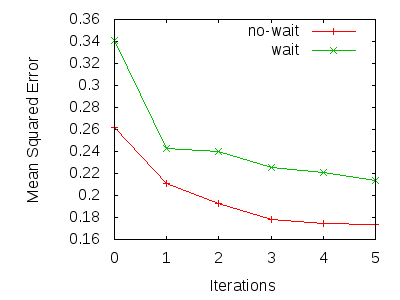
\includegraphics[width=0.7\textwidth]{output.png}
%\end{centering}
%\label{fig:toyData}
%\caption{A toy data example run for LDA formulation}
%\end{figure}


\comment{\\ Comparison with PSGD on the speed and accuracy of convergence (Do
we compare on the original objective or the new objective)\\}

%\vspace{-0.2cm}
%\subsection{Qualitative results on latent space models}
%\vspace{-0.2cm}
%\comment{\\We do both for MMSB and LDA}
%\comment{\\Qirong and Alex think that we should include symmetric matrix
%factorization as well as it shows the scheduling strategy when things are not cleanly seperated.}

\begin{table*}[t]
\vspace{-0.4cm}
\centering
\scriptsize
    \setlength{\tabcolsep}{4.5pt}
\begin{tabular}{|c|c|c|c|c|c|c|c|c|c|}
\hline
Topic 1 & Topic 2 & Topic 3 & Topic 4 & Topic 5 & Topic 6 & Topic 7 & Topic 8 & Topic 9 & Topic 10\\
\hline
micchelli & kirchoff & iris & texture & maintained & foveal & neglect & microchip & microchip & indexed \\
phased & endmember & chou & creasing & cknn & cotterill & rho & ecc & sondik & originate \\
alike & sander & consideration & descending & spotlight & endmember & micchelli & stabilizing & unfolded & release \\
umli & fre & retinotopic & locate & subgoal & retinotopic & cepstrum & manifold & eeg & occurred \\
saliencies & triangulated & falling & sociated & treatment & easiest & interference & anton & shortest & multicollinearity \\
spotlight & sep & pca & perceptual & robot & bbn & indiveri & tour & resembling & multitask \\
gammon & assumption & eval & saund & hitting & chi & sharpe & unconditional & inhibition & dendritic \\
sdti & hole & winner & onset & normalization & lesson & leaning & reside & cell & helpful \\
viewer & suzanna & segmentation & lrta & fish & refractory & packet & patient & nearest & depth \\
riken & denote & cole & mary & searching & chip & sensitivity & arethor & neighbor & partic \\
\hline
\end{tabular}
\vspace{-0.4cm}
\caption{\small A selection of topics from the NIPS corpus.
}
\label{tab:nips_lda}
\vspace{-0.4cm}
\end{table*}


% No need for a separate eesults section. State your conclusions inline with the experiments
%\section{Results, Analysis and Discussion}

% Qirong: Conclusions are a waste of space, don't bother
%\section{Conclusion}


{
\small
\bibliography{biblio}
\bibliographystyle{plain}
}

\end{document}
